\documentclass[12pt,a4paper,ngerman]{article}
\usepackage[german,ngerman]{babel} % sorgt dafür, dass "Inhaltsverzeichnis" auf deutsch angezeigt wird, und wahrscheinlich noch ein paar andere Sachen auch
\usepackage{amsmath}
\usepackage{amsfonts}
\usepackage{amssymb}
\usepackage[top=2.5cm, bottom=2.5cm, outer=4cm, inner=2.5cm, heightrounded, marginparwidth=2.5cm, marginparsep=0.5cm]{geometry}
\usepackage{graphicx}

\usepackage{wrapfig, ragged2e}
\usepackage[font=small,labelfont=bf]{caption} % Bildunterschriftdesign
\usepackage{float}
\usepackage{fontspec,xunicode}  % dadurch kann man auch äöü direkt im text eingeben

%\usepackage[utf8]{inputenc}



\setmainfont{Arial}

\setcounter{secnumdepth}{4} % erlaubt Unter-Unter-Kapitel

% folgendes macht automatisch Links im Inhaltsverzeichnis des Pdfs, die direkt zum Unterkapitel führen
\usepackage[colorlinks,pdfpagelabels,pdfstartview = FitH,bookmarksopen = true,
bookmarksnumbered = true,linkcolor = black,plainpages = false,hypertexnames = false,
citecolor = black] {hyperref}


% für Zitate
\usepackage[style=numeric, backend=bibtex]{biblatex}
\addbibresource{Quellenverzeichnis}  % Bibtex-Datei wird schon in der Preambel eingebunden

% Sachen wegen Literaturverzeichnis
\usepackage{url}
\newcommand*\oldurlbreaks{}
\let\oldurlbreaks=\UrlBreaks
\renewcommand{\UrlBreaks}{\oldurlbreaks\do\\}
%\renewcommand{\UrlBreaks}{\oldurlbreaks\do\a\do\b\do\c\do\d\do\e%
%  \do\f\do\g\do\h\do\i\do\j\do\k\do\l\do\m\do\n\do\o\do\p\do\q%
%  \do\r\do\s\do\t\do\u\do\v\do\w\do\x\do\y\do\z\do\?\do\&}
\usepackage{hyperref} 


 \usepackage[disable]{todonotes}
\begin{document}
\setlength{\parindent}{0pt} % kein Einzug bei Absatzanfang

\begin{titlepage}
\begin{flushleft}
\begin{Huge}
\textbf{Hochschule München}
\par\medskip
Projektarbeit Wackelroboter
\end{Huge}
\begin{large}
\par\bigskip
\par\bigskip
\par\bigskip
\par\bigskip
\begin{figure}[h]
\centering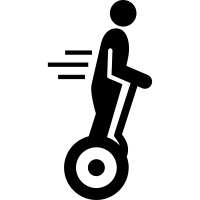
\includegraphics[width=0.3\textwidth]{images/segwayIcon.png}

% würde eine Bildunterschrift erzeugen
%\caption[Eintrag im Abbildungsverzeichnis]{}
\end{figure}

\par\bigskip
\par\bigskip
\par\bigskip
\par\bigskip

\begin{description}
\item[Autoren]~\par
\begin{itemize}
\item Valentyn Chepil
\item Stephan Morongowski
\item Severin Schendel
\item Aleksandar Stoiljkovic
\item Timo Veit
\end{itemize}
\end{description}

%Autoren: Valentyn Chepil, Stephan Morongowski, Severin Schendel, Aleksandar Stoiljkovic, Timo Veit

\begin{description}
\item[Betreuer]~\par
\begin{itemize}
\item Prof. Dr. Norbert Nitzsche
\end{itemize}
\end{description}


\end{large}
\end{flushleft}


%\centering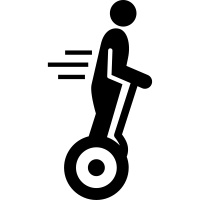
\includegraphics{images/segwayIcon.jpg}
\vfill % Fill the rest of the page with whitespace
\end{titlepage}


%\pdfbookmark[1]{Inhaltsverzeichnis}{toc}

\tableofcontents
\newpage



% hier werden alle Extradateien eingebunden
\input{motivation.tex}
\newpage
\section{Navigation}

Wie navigiert man in der Ebene? Hier ein Beispiel für ein Zitat: Vgl. \cite{bildungAtmosphaere}

\subsection{Sensorik}
Zur Verfügung stehen folgende Sensoren:
\begin{itemize}
\item Gyros in allen drei Raumachsen
\item Beschleunigungssensoren in allen drei Raumachsen
\item Inkrementalgeber der Räder
\item Ultraschallsensoren
\end{itemize}

\subsection{Inkrementalgeber}

Zur Bestimmung der Position des Roboters in einem festen Koordinatensystem können die Inkrementalgeber der Antriebsmotoren benutzt werden.
Sie liefern pro Umdrehung 1024 Impulse. Das ergibt bei einem Raddurchmesser von 8 cm eine Auflösung von ca. 0,5 mm pro Strich. 

\begin{figure}[h]  % [h] bedeutet, dass das Bild genau an dieser Stelle im Text erscheint
\centering\includegraphics[width=0.8\textwidth]{images/Kurvenkinematic.eps}
\caption{Rotation um den Momentanpol \newline (Quelle: eigene Darstellung)}
\label{kurvenkinematik}
\end{figure}

Zur Ermittlung der aktuellen Position ist in Abbildung \ref{kurvenkinematik} die Kinematik einer Kurvenfahrt dargestellt, betrachtet für einen gedanklich sehr kleinen Zeitabschnitt. In diesem wird angenommen, dass die Geschwindigkeiten \(v_1\) und \(v_2\) beider Räder konstant bleiben. Dies sorgt fürdie Vereinfachung, dass der Roboter sich auf einer Kreisbahn um einen für die betrachtete Zeitspanne konstanten Momentanpol bewegt. Im Folgenden sind die durch den Inkrementalgeber erfassten Bogenlängen mit arc bezeichnet.
Es gilt:
\begin{flalign}
    % durch das & Zeichen werden alle Gleichungen an diesem Punkt ausgerichtet
	arc_{R1} &  = \Delta\varphi\cdot r_{R1} 
	\label{eq:bogenmaß_1} \\
	arc_{R2} & = \Delta\varphi\cdot r_{R2} 
	\label{eq:bogenmaß_2} \\
	r_{R1} & = r_{R2}  + l_a 
	\label{eq:achsZuMomentanpol} \\
	\Delta arcs & = arc_{R2} - arc_{R1}
	\label{eq:arcsDef}
\end{flalign}

Aus \eqref{eq:bogenmaß_1}, \eqref{eq:bogenmaß_2}, \eqref{eq:achsZuMomentanpol} und \eqref{eq:arcsDef} folgt:
% hier keine Leerzeile machen, sonst wird der Abstand ganz groß
\begin{flalign}
    \Delta\varphi & = \frac{1}{l_a} \cdot \Delta arcs
	\label{eq:deltaPhi}
\end{flalign}
Durch Aufsummieren von \(\Delta\varphi\) nach jeder Auswertung der Inkrementalgeber kann somit ein ungefährer Absolutwinkel der Roboterachse zu einem festen KS berechnet werden.

\begin{lstlisting}[language=C++, caption=deadReckonTotalPhi]
float deadReckonTotalPhi(int inkLeft, int inkRight) {
	static float totalPhi = 0.0f;
	totalPhi = totalPhi + 1/l_a * (inkRight - inkLeft);
	return totalPhi;
}
\end{lstlisting}

Zur Bestimmung des Schwerpunktes in xy-Koordinaten wird die Verschiebung von 
\(S_0\) zu \(S_1\) mit trigonometrischen Funktionen berechnet und anschließend aufsummiert.



\newpage
\renewcommand\refname{Literaturverzeichnis}
\printbibliography 
\listoffigures
\end{document}
